\section{Realtime-Opeartionsystem}

\subsection{Kernel}

\textit{
    Following can be leveraged from using RTOS:
}

\begin{itemize}
    \item{\textit{
        \textbf{parallelism} of  a program
    }}
    \item{\textit{
        \textbf{Simplifing} the program, only using ISR-concepts can make it complicated
    }}
\end{itemize}

\begin{tabular}{lp{0.4\textwidth}}
    Realtime    & \textit{Defined \textbf{reaction time} to an event} \\
                & \textit{(hard/soft real time: result/reaction)} \\
    RT-OS       & \textit{Real-Time Operating System} \\
    $\mu$C/OS-II  & \textit{uC Operating System, product that we use} \\
    Kernel      & \textit{Basic functions of MT-OS (Multitask-OS)} \\
    Scheduler   & \textit{Divides/assigns CPU-ressources to the tasks} \\
\end{tabular}

\subsection{Scheduler}

\textit{There are different strategies how resources are shared and managed by the scheduler:}

\begin{tabular}{lp{0.3\textwidth}}
    Strategies      & \textit{First-Come First-Serve} \\
                    & \textit{Shortest Job First} \\
                    & \textit{\textbf{Round Robin} (equal time slices for each task)} \\
                    & \textit{\textbf{Priority based} (different task priorities)} \\
    Preemptive      & \textit{
                        Scheduler takes the system ressources from the
                        Task (Process) (Task with higher Priority,
                        Timeslicing…)
                    } \\
    Cooperative  & \textit{The task hands the systemressources over by itself} \\
\end{tabular}

\subsection{non-reentrant / reentrant}

\textit{
    Non-reentrant function can not be shared, they have a state. \newline
    Reentrant functions can be reentred multible times (Tasks can share code)
}

\subsection{RTOS Task}

\begin{wrapfigure}{l}{0.2\textwidth}
    \centering
    \vspace{-20pt}
    \hspace{-20pt}
    \vspace{-10pt}
    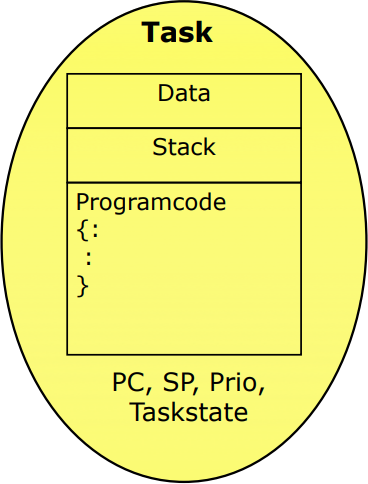
\includegraphics[width=0.2\textwidth]{rtos-task.png}
    \hspace{-50pt}
\end{wrapfigure}

\textit{
    Every task contains its own: \newline
    \textbf{Data}, \textbf{Stack}, \textbf{Programmcode},
    \textbf{PC}, \textbf{SP} \newline
    It always is an \textbf{endless loop or quits itself}
    -> no return value.
    there are \textbf{Max. 255 Tasks}. \newline
    \textbf{Task-ID} = \textbf{Task-Priority} \newline
    \newline
}

\subsection{Task States}

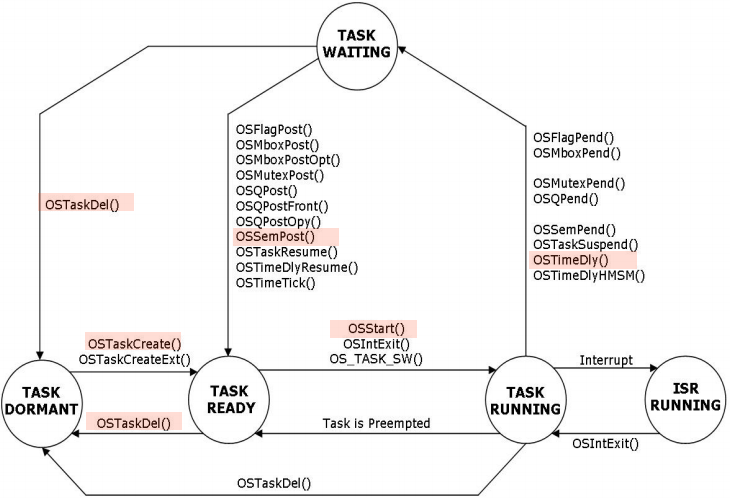
\includegraphics[width=0.5\textwidth]{rtos-task-states.png}

\begin{tabular}{lp{0.4\textwidth}}
    Waiting & \textit{
        The Task \textbf{waits} for an \textbf{event} (Timer, Semaphor,
        Input,… ). As soon the event happens, the task is set
        to the ready state.
    } \\
    Ready   & \textit{
        The task is \textbf{ready for running} and waits until it gets
        activated by the scheduler.
    } \\
    Dormant & \textit{
        A Task in the dormant state can not be assigned by
        the scheduler (the memory is not deleted).
    } \\
    Running & \textit{
        The task is running (CPU is used by this task).
    } \\
    ISR-Running & \textit{
        As soon an interrupt happens, the OS changes the
        state to ISR-Running (to a depth of 255).
    }
\end{tabular}

\subsection{Create task}

\begin{lstlisting}
OSTaskCreate(void (*task)(void *pd), void *pdata, OS_STK *ptos, INT8U prio)
\end{lstlisting}

\textit{
    \textbf{pd}: Pointer to the task code \newline
    \textbf{pdata}: Pointer to any arguments with for the task code \newline
    \textbf{ptos}: Pointer pointing to the end of the task stack \newline
    \textbf{prio}: ID and prio of the task, smaller = more prio
}

\textit{
    \textbf{Before} the execution of \textbf{OSStart(...)} there must have been
    created \textbf{at least 1 Task}\newline
    Task is \textbf{always} "\textbf{void}" (no return values!)\newline
    Task: either endless loop, or selfdeleting at the end\newline
    Idle Task => Stack Usage!!!
}

\subsection{RTSO Timer}

\textit{
    On \textbf{uCOS-II}: 1 unit is \textbf{20 ms} (configurable = 1 Tick)
}

\begin{lstlisting}
// Set Timer to 2000ms (2s)(100 x 20ms)
OSTimeDly(100);
// Set Timer to 1h
OSTimeDlyHMSM(1,0,0,0);
// Resume with priority 5 Task, also when the timer of this task has not ran down yet
OSTimeDlyResume(5);
// Number of Ticks since OSStart() or OSTimeSet()
OSTimeGet();
OSTimeSet();
\end{lstlisting}

\subsection{Contextswitch}

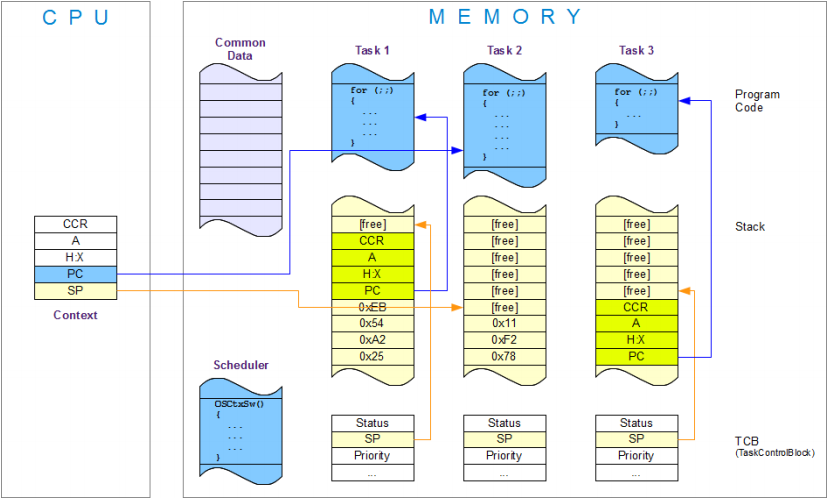
\includegraphics[width=0.5\textwidth]{rtos-context-switch.png}

\subsection{Parallelism}

\textit{
    \textbf{Tasks} that are dependent from each other must
    \textbf{cooperate}. We can differenciate between:
}

\begin{tabular}{ll}
    \textbf{Synchronisation} & \\
    \textit{\textbf{Semaphore}} & \textit{was Train Signal} \\
    \textit{\textbf{Mutex}}     & \textit{\textbf{Mut}ual \textbf{ex}clusion} \\
    \textit{\textbf{Flags}}     & \textit{Signaling Flags} \\
    \textbf{Communication} & \\
    \textit{\textbf{Mailbox}} & \\
    \textit{Message \textbf{Queues}} & \\
\end{tabular}

\textit{
    \newline
}
\begin{itemize}
    \item{\textit{
        Tasks can simply communicate over \textbf{data structures}
    }}
    \item{\textit{
        Example: Time - h and min values stored each as
        global 8-bit variables (1 task Wr / 1 task Rd)
    }}
    \item{\textit{
        For coherent data \textbf{Mutual exclusion} is imminent
    }}
    \item{\textit{
        Methods for Mutual Exclusion are; \textbf{Disable Scheduler and Interrupts},
        \textbf{Semaphors}
    }}
\end{itemize}

\subsubsection{Semaphore}

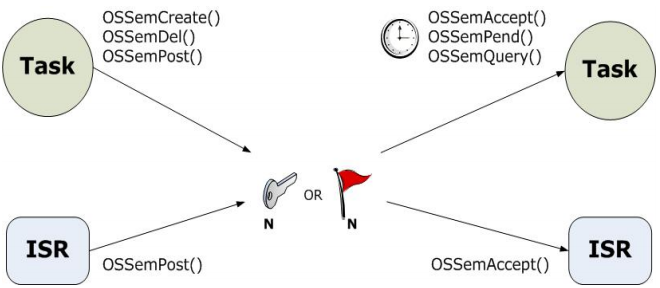
\includegraphics[width=0.5\textwidth]{rtos-semaphore.png}

\begin{lstlisting}
// Define Semaphore
OS_EVENT *sem_X;
// Create Semaphore and set to 100
sem_X = OSSemCreate(100);
INT8U err;
// Wait for free Semaphore Timeout = 0 (endless) critical Code...
OSSemPend(sem_X, 0, &err);
// Free Semaphore
OSSemPost(sem_X);
\end{lstlisting}

\subsubsection{Mutex}

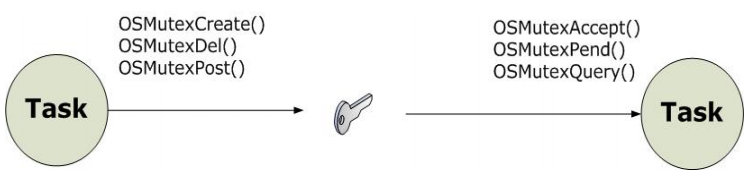
\includegraphics[width=0.5\textwidth]{rtos-mutex.png}

\begin{lstlisting}
// Define Mutex
OS_EVENT *mut_X;
INT8U err;
// Create Mutex with Priority (prio is overtaken when mutex gets owned)
mut_X = OSMutexCreate(9, &err)
// Wait for freeing of Mutex, Timeout = 0 (endless)
OSMutexPend(mut_X, 0, &err);
// Free Mutex
OSMutexPost(mut_X);
\end{lstlisting}

\subsubsection{Flags}

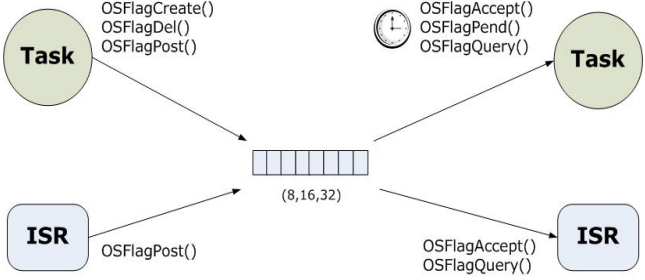
\includegraphics[width=0.5\textwidth]{rtos-flags.png}

\begin{lstlisting}
// Define Flag group
OS_FLAG_GRP *fg_x;
INT8U err;
// Create Flag group and init.
fg_x = OSFlagCreate(0x00, &err);
OS_Flags value;
// wait until BIT0 and BIT1 get set in the Flag group or the timeout expires
Value = OSFlagPend(fg_x, 0x01+0x02, OS_FLAG_WAIT_SET_ALL, 10, &err);
\end{lstlisting}

\subsubsection{Mailbox}

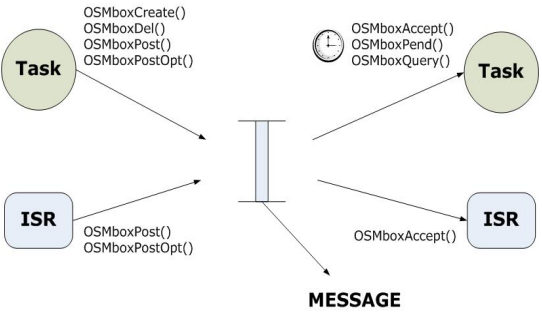
\includegraphics[width=0.5\textwidth]{rtos-mailbox.png}

\begin{lstlisting}
// Define Mailbox
OS_EVENT *mBox;
// Create empty Mailbox
mBox = OSMBoxCreate((void *)0);
// Store Message in Mailbox
OSMBoxPost(mBox, &message);
INT8U err;
// Wait for a Message
OSMBoxPend(mBox, 0, &err);
\end{lstlisting}

\subsubsection{Queue}

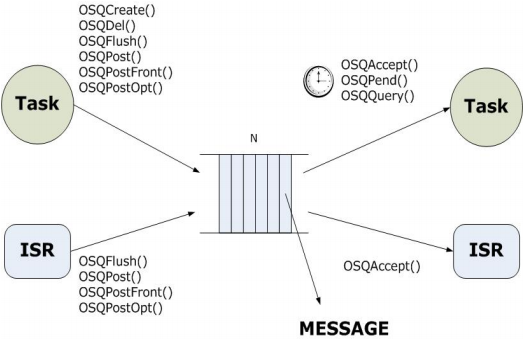
\includegraphics[width=0.5\textwidth]{rtos-queue.png}

\begin{lstlisting}
// Define Message-Queue
OS_EVENT *queue;
// Array for Queue-Data
void *data[10];
// Create Message-Queue
queue = OSQCreate(data, 10);
// Add Message in Queue
INT8U err = OSQPost(queue, &message);
// Wait for a Message
void *msg = OSQPend(queue, 0, &err);
\end{lstlisting}

\subsection{Priority Inversion}

\textit{
    A low priority task blocks a higher priority task while
    accessing a common ressource. This can happen while semaphores
    are used. Mutex have a solution, they will execute the part when
    the mutex is borrowed in an different priority, usually higher then
    everything else.
}

\subsection{Code}

\begin{lstlisting}
// stacksize for all the task, can be differntly sized
#define TASK_STK_SIZE 128

#define PRIO_INIT           0
// always max. priority for the init task.
#define PRIO_BLINK_1        2
#define PRIO_BLINK_2        3
// mutex can be used to have different prios
// for the time the mutex is used
#define PRIO_MUT_DISP       1

// Array of type OS_STK stackmemory. needs to be done for every task
OS_STK InitTaskStack[TASK_STK_SIZE];
OS_STK Blink1Stack[TASK_STK_SIZE];
OS_STK Blink2Stack[TASK_STK_SIZE];

OS_EVENT *Mut_Displ;
OS_EVENT *Sem_Displ;


void Blink1(void *pdata)
{
    uint8 color,i,res;

    color=SSD1307_PIXEL_BLACK;
    (void)pdata;
    for(;;)
    {
        for(i=0;i<96;i++)
        {
            //OSMutexPend(Mut_Displ, 0, &res);
            OSSemPend(Sem_Displ, 0, &res);
                GDisp1_DrawVLine(i,2,5,color);
                SSD1307_UpdateFull();
            //(void)OSMutexPost(Mut_Displ);
            (void)OSSemPost(Sem_Displ);

            PTFD_PTFD1 = !PTFD_PTFD1;	//Blinking LED
            OSTimeDly(20);
        }
        if(color==SSD1307_PIXEL_BLACK)
        {
            color=SSD1307_PIXEL_WHITE;
        }
        else
        {
            color=SSD1307_PIXEL_BLACK;
        }
    }
}

void Blink2(void *pdata)
{
    // same as blink1 with differnt OSTimeDly(46);
}

void InitTask(void* pdata)
{
    (void)pdata; // surpress compiler warning
    OSTimerInit(); // configer and start timer
    // ...
    // space for more initialisation
    // ...

    (void)OSTaskCreate(Blink1, (void*)0, &Blink1Stack[TASK_STK_SIZE-1], PRIO_BLINK_1);
    (void)OSTaskCreate(Blink2, (void*)0, &Blink2Stack[TASK_STK_SIZE-1], PRIO_BLINK_2);

    (void)OSTaskDel(OS_PRIO_SELF); // close init task
}
void main(void)
{
    OSInit(); // OS initialisieren
    // Task Ptr, Argument Ptr, Stack Ptr, Task Id = Prio
    OSTaskCreate(InitTask, (void*)0, &InitTaskStack[TASK_STK_SIZE-1], PRIO_INIT);
    // Vor Aufruf von OSStart(..) muss mindestens 1 Task erzeugt sein
    OSStart(); // start OS
}
\end{lstlisting}